\documentclass[12pt]{article}
\usepackage[dvips]{epsfig}
\usepackage{color}
\usepackage{url}
\usepackage[colorlinks=true]{hyperref}

\begin{document}

\section*{GENESIS: Documentation}

\section*{RTXI ``injector'' Module Validation}
A step by step validation procedure for the RTXI ``injector'' module. This procedure should be run prior to connecting RTXI to an external amplifier. It enables the correct application of scaling factors to match RTXI output and input to the units employed in a source file containing a stimulus signal. The following steps should be initiated from the desktop of your machine that has RTXI installed. 

\subsection*{Validation Procedure}

\subsubsection*{Activation of stimulus signal}

\begin{enumerate}
	\item Start a terminal window.
	\item In the terminal window enter {\tt rtxi}.
	\item From the RTXI {\bf Control} drop-down menu select {\bf Plugin Loader}.
	\item From the {\bf Open File} dialog box select {\bf injector.so}.
	\item In the new {\bf Open File} dialog box go to {\tt /home/Suterlab}.

	\begin{enumerate}
		\item Select {\bf Desktop}.
		\item Select {\bf dynamic--clamp}.
		\item Select {\bf stim-src}.
		\item Select validation input file {\tt Offset400.txt}.
	\end{enumerate}

	\item In the Injector control window popup
	\begin{enumerate}
		\item Set {\bf Gain GABA} to {\tt 1e9}.
		\item Set {\bf Global Offset} to {\tt 0}.
		\item Set {\bf GABA Enabled?} to {\tt 1}.
		\item Click the {\bf Modify} button at the bottom of the panel. This will cause the altered values 
			to change color from \textcolor{red}{red} to black.
		\item Click the {\bf Pause} button.
	\end{enumerate}
\end{enumerate}
The square pulse waveform read from the input file ({\tt Offset400.txt}) is now being generated internally within RTXI by the {\tt injector.so} plugin.

\subsubsection*{Visualizing the internally generated signal}

\begin{enumerate}
	\item From the RTXI {\bf Control} drop-down menu select {\bf Oscilloscope}. (The oscilloscope 
		window should appear.)
	\item Right click on the oscilloscope window, select {\bf Properties}.
	\item In the oscilloscope properties dialog box set the {\bf Channel} drop-down boxes to the values:
		\begin{tabular}{ l c r }
			 {\bf Injector2} & {\bf Output} & {\bf GoutGABA}
		 \end{tabular}
	\item Click the {\bf Active} button at right hand end of the {\bf Channel} boxes.
 	\item Set the {\bf Display Properties Scale} to 200\,mV/div.
 \item Click the {\bf Apply} button at the bottom left of the oscilloscope properties dialog box.

\end{enumerate}
You should now see the generated square-pulse  with an amplitude of 2 divisions on the RTXI oscilloscope screen. The amplitude is equivalent to 400\,mV (see the scale in the bottom left of the oscilloscope window). Each pulse is 1\,ms in duration to give 5 pulses per 5\,ms division (Scale on bottom right hand side of the oscilloscope window gives the absolute duration of the window).

\subsubsection*{Connect internally generated RTXI signal to the DAQ output}

\begin{enumerate}
	\item Select {\bf Connector} from the RTXI {\bf Control} drop-down menu.
	\item In the {\bf Connector} dialog box set the {\bf Output Block} to {\bf Injector2}, the {\bf Input Block} 
		to the DAQ board name (here {\bf NI\,PCIe--6251\,14}), and the {\bf Channel} to {\bf Analog 
		Output 0}.
	\item Click the right facing arrow ``$==>$'' to connect the RTXI output block to the DAQ board input block.
\end{enumerate}

\subsubsection*{Enable the analog output of the DAQ}

\begin{enumerate}
	\item From the RTXI {\bf Control} drop-down menu select {\bf System Control}  and check the {\bf 
		Device} is the DAQ board (here {\bf NI\,PCIe--6251\,14}).
	\item Set the {\bf Analog Channel} to {\bf Output channel number 0}.
	\item Click the {\bf Active} button on the right hand side.
	\item Click the {\bf Apply} button at the bottom left hand side of the panel.
	\item Configure the hardware oscilloscope to 5\,ms and 200\,mV.
\end{enumerate}

\subsubsection*{Configure RTXI software oscilloscope to monitor incoming signal}

\begin{enumerate}
	\item From the RTXI {\bf Control} drop-down menu select {\bf Oscilloscope}.
	\item Right click on the oscilloscope panel and select {\bf Oscilloscope Properties}.
	\item Select:
		\begin{tabular}{ l c r }
			{\bf NI\,PCIe--6251\,14} & {\bf Output} & {\bf Analog Input 0}
		\end{tabular}
	\item Click to select {\bf Active} at right hand end.
	\item Set {\bf Display Property Scale} to 200\,mV/div.
	\item Select {\bf Line Property Color ``\textcolor{blue}{blue}''}.
	\item Click {\bf Apply} button on lower left hand side of the oscilloscope panel.
\end{enumerate}

\subsubsection*{Enable the input signal from the DAQ}

\begin{enumerate}
	\item From the RTXI {\bf Control} drop-down menu select {\bf System Control}
	\item Select {\bf Device  NI\,PCIe--6251\,14} board.
	\item Select: {\bf Analog Input Channel Input 0}.
	\item Click {\bf Active} button at right hand end.
	\item Click {\bf Apply} button at bottom left hand side of panel.
	\item The RTXI input signal (identical to the output signal for this validation test) should now appear 
	on the screen of the RTXI software oscilloscope.
	\item We measure $\approx$\,0.1\,ms between the input and output traces of the signal.
\end{enumerate}

\subsection*{Hardware Cabling and Switches}

\begin{figure}[h]
  \centering
    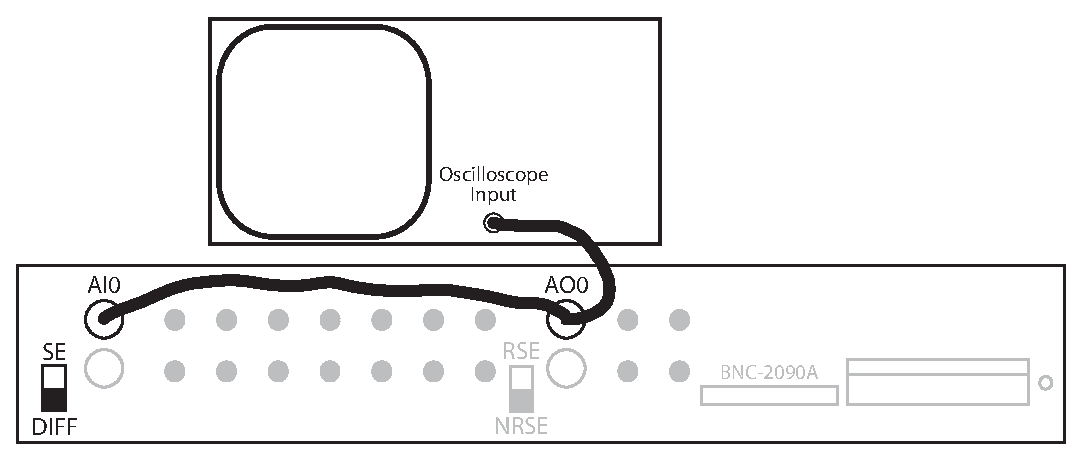
\includegraphics[scale=0.75]{figures/rtxi-connector-backpanel.eps}
    \caption{Cabling for RTXI ``injector'' module validation. {\tt AI0}: Analog input zero (0), {\tt AO0}: Analog output zero (0). SE/DIFF switch should be set to DIFF. In DIFF mode the RSE/NRSE switch has no effect.}
  \label{fig:rtxi-inj}
\end{figure}

\end{document}
